\documentclass{article}

\usepackage{enumerate}
\usepackage{amsmath,amsthm,amssymb}
\usepackage{tikz}
\usepackage{pgfplots}
\usepackage{multicol}
%\pgfplotsset{compat=newest}

\usepackage[margin=1in]{geometry}

\begin{document}

\noindent \textbf{Name:}\underline{\hspace{2in}} \hfill \textbf{Handout: August 28}
\vspace{1em}

The following is the graph of a \emph{Logistic Growth Curve} $L(x) = 1/(1 + e^{-x})$. 
\begin{center}
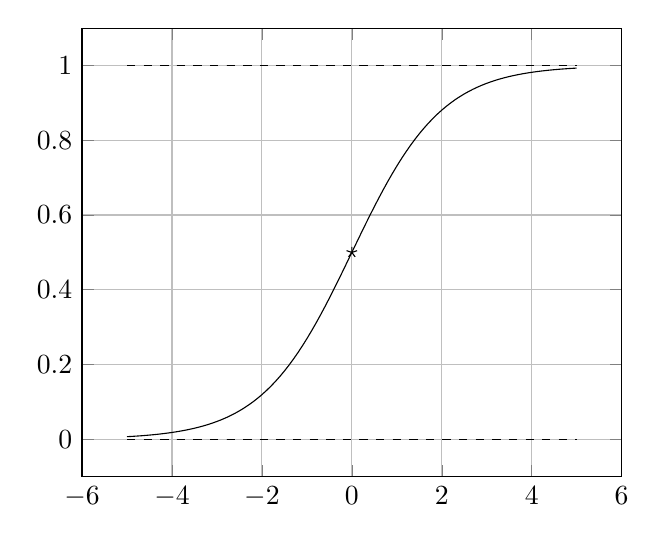
\begin{tikzpicture}
\begin{axis}[grid=both]%[enlargelimits=false]
  \addplot [domain=-5:5, samples=101,unbounded coords=jump]{1/ (1 + e^-x)};
  \addplot [samples=10, dashed] {1};
  \addplot [samples=10, dashed] {0};
  \addplot coordinates{(0,0.5)};
\end{axis}
\end{tikzpicture}
\end{center}
The logistic growth curve has horizontal asymptotes at $y = 0$ and $y=1$, as is indicated by the dashed lines. Furthermore, its \emph{inflection point} is the point $(0,0.5)$.

\begin{enumerate}
\item What are the horizontal asymptotes and inflection points of the following functions? (Show your work!)
  \begin{enumerate}
  \item $L(-1.5 x + 3)$
    \vspace{1.5in}
  \item $-1.5 \cdot L(x) + 3$
    \vspace{1.5in}
  \item $-1.5 \cdot L( -1.5 x + 3) + 3$
  \end{enumerate}
\pagebreak
\item The following is a graph of the \emph{natural logarithm} function $\ln(x)$. Its domain is $(0,\infty)$.
  \begin{center}
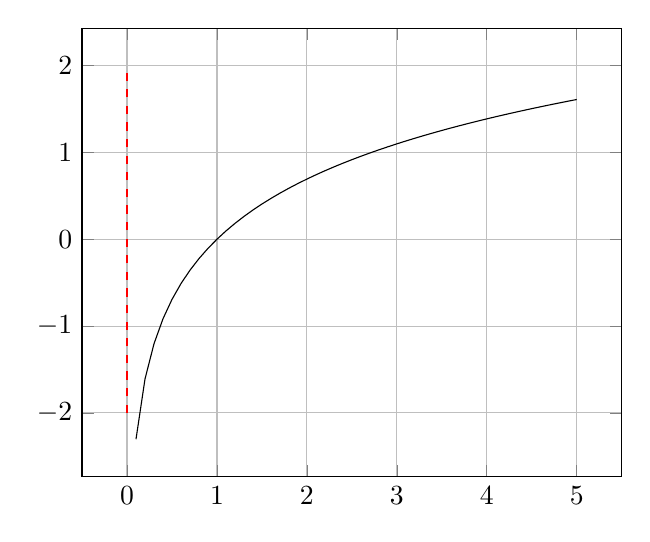
\begin{tikzpicture}
\begin{axis}[grid = both]%[enlargelimits=false]
  \addplot [domain=-5:5, samples=101,unbounded coords=jump]{ln(x))};
  \addplot +[mark=none, dashed] coordinates {(0, -2) (0, 2)};
\end{axis}
\end{tikzpicture}
\end{center}
\begin{enumerate}
\item Give the domain of the following functions:
  \begin{multicols}{2}
  \begin{enumerate}
  \item $\ln(1-x)$
    \vspace{1in}
  \item $\ln(5 + x)$
    \vspace{1in}
  \item $\ln(1) - \ln(x)$
    \vspace{1in}
  \item $1 - \ln(x)$
  \end{enumerate}
\end{multicols}
\vspace{1in}

\item What is the domain of $\ln(|x|)$?
  \vspace{1in}
\item What is the domain of $\sqrt{\ln(x)}$?
\end{enumerate}

\end{enumerate}
\end{document}
